
%% bare_conf.tex
%% V1.3
%% 2007/01/11
%% by Michael Shell
%% See:
%% http://www.michaelshell.org/
%% for current contact information.
%%
%% This is a skeleton file demonstrating the use of IEEEtran.cls
%% (requires IEEEtran.cls version 1.7 or later) with an IEEE conference paper.
%%
%% Support sites:
%% http://www.michaelshell.org/tex/ieeetran/
%% http://www.ctan.org/tex-archive/macros/latex/contrib/IEEEtran/
%% and
%% http://www.ieee.org/

%%*************************************************************************
%% Legal Notice:
%% This code is offered as-is without any warranty either expressed or
%% implied; without even the implied warranty of MERCHANTABILITY or
%% FITNESS FOR A PARTICULAR PURPOSE!
%% User assumes all risk.
%% In no event shall IEEE or any contributor to this code be liable for
%% any damages or losses, including, but not limited to, incidental,
%% consequential, or any other damages, resulting from the use or misuse
%% of any information contained here.
%%
%% All comments are the opinions of their respective authors and are not
%% necessarily endorsed by the IEEE.
%%
%% This work is distributed under the LaTeX Project Public License (LPPL)
%% ( http://www.latex-project.org/ ) version 1.3, and may be freely used,
%% distributed and modified. A copy of the LPPL, version 1.3, is included
%% in the base LaTeX documentation of all distributions of LaTeX released
%% 2003/12/01 or later.
%% Retain all contribution notices and credits.
%% ** Modified files should be clearly indicated as such, including  **
%% ** renaming them and changing author support contact information. **
%%
%% File list of work: IEEEtran.cls, IEEEtran_HOWTO.pdf, bare_adv.tex,
%%                    bare_conf.tex, bare_jrnl.tex, bare_jrnl_compsoc.tex
%%*************************************************************************

% *** Authors should verify (and, if needed, correct) their LaTeX system  ***
% *** with the testflow diagnostic prior to trusting their LaTeX platform ***
% *** with production work. IEEE's font choices can trigger bugs that do  ***
% *** not appear when using other class files.                            ***
% The testflow support page is at:
% http://www.michaelshell.org/tex/testflow/



% Note that the a4paper option is mainly intended so that authors in
% countries using A4 can easily print to A4 and see how their papers will
% look in print - the typesetting of the document will not typically be
% affected with changes in paper size (but the bottom and side margins will).
% Use the testflow package mentioned above to verify correct handling of
% both paper sizes by the user's LaTeX system.
%
% Also note that the "draftcls" or "draftclsnofoot", not "draft", option
% should be used if it is desired that the figures are to be displayed in
% draft mode.
%
\documentclass[10pt, conference, compsocconf]{IEEEtran}
% Add the compsocconf option for Computer Society conferences.
%
% If IEEEtran.cls has not been installed into the LaTeX system files,
% manually specify the path to it like:
% \documentclass[conference]{../sty/IEEEtran}





% Some very useful LaTeX packages include:
% (uncomment the ones you want to load)


% *** MISC UTILITY PACKAGES ***
%
%\usepackage{ifpdf}
% Heiko Oberdiek's ifpdf.sty is very useful if you need conditional
% compilation based on whether the output is pdf or dvi.
% usage:
% \ifpdf
%   % pdf code
% \else
%   % dvi code
% \fi
% The latest version of ifpdf.sty can be obtained from:
% http://www.ctan.org/tex-archive/macros/latex/contrib/oberdiek/
% Also, note that IEEEtran.cls V1.7 and later provides a builtin
% \ifCLASSINFOpdf conditional that works the same way.
% When switching from latex to pdflatex and vice-versa, the compiler may
% have to be run twice to clear warning/error messages.






% *** CITATION PACKAGES ***
%
%\usepackage{cite}
% cite.sty was written by Donald Arseneau
% V1.6 and later of IEEEtran pre-defines the format of the cite.sty package
% \cite{} output to follow that of IEEE. Loading the cite package will
% result in citation numbers being automatically sorted and properly
% "compressed/ranged". e.g., [1], [9], [2], [7], [5], [6] without using
% cite.sty will become [1], [2], [5]--[7], [9] using cite.sty. cite.sty's
% \cite will automatically add leading space, if needed. Use cite.sty's
% noadjust option (cite.sty V3.8 and later) if you want to turn this off.
% cite.sty is already installed on most LaTeX systems. Be sure and use
% version 4.0 (2003-05-27) and later if using hyperref.sty. cite.sty does
% not currently provide for hyperlinked citations.
% The latest version can be obtained at:
% http://www.ctan.org/tex-archive/macros/latex/contrib/cite/
% The documentation is contained in the cite.sty file itself.






% *** GRAPHICS RELATED PACKAGES ***
%
\ifCLASSINFOpdf
  % \usepackage[pdftex]{graphicx}
  % declare the path(s) where your graphic files are
  % \graphicspath{{../pdf/}{../jpeg/}}
  % and their extensions so you won't have to specify these with
  % every instance of \includegraphics
  % \DeclareGraphicsExtensions{.pdf,.jpeg,.png}
\else
  % or other class option (dvipsone, dvipdf, if not using dvips). graphicx
  % will default to the driver specified in the system graphics.cfg if no
  % driver is specified.
  % \usepackage[dvips]{graphicx}
  % declare the path(s) where your graphic files are
  % \graphicspath{{../eps/}}
  % and their extensions so you won't have to specify these with
  % every instance of \includegraphics
  % \DeclareGraphicsExtensions{.eps}
\fi
% graphicx was written by David Carlisle and Sebastian Rahtz. It is
% required if you want graphics, photos, etc. graphicx.sty is already
% installed on most LaTeX systems. The latest version and documentation can
% be obtained at:
% http://www.ctan.org/tex-archive/macros/latex/required/graphics/
% Another good source of documentation is "Using Imported Graphics in
% LaTeX2e" by Keith Reckdahl which can be found as epslatex.ps or
% epslatex.pdf at: http://www.ctan.org/tex-archive/info/
%
% latex, and pdflatex in dvi mode, support graphics in encapsulated
% postscript (.eps) format. pdflatex in pdf mode supports graphics
% in .pdf, .jpeg, .png and .mps (metapost) formats. Users should ensure
% that all non-photo figures use a vector format (.eps, .pdf, .mps) and
% not a bitmapped formats (.jpeg, .png). IEEE frowns on bitmapped formats
% which can result in "jaggedy"/blurry rendering of lines and letters as
% well as large increases in file sizes.
%
% You can find documentation about the pdfTeX application at:
% http://www.tug.org/applications/pdftex





% *** MATH PACKAGES ***
%

\usepackage[cmex10]{amsmath}
\usepackage{tikz}

\definecolor{bluekeywords}{rgb}{0,0,1}
\definecolor{greencomments}{rgb}{0,0.5,0}
\definecolor{redstrings}{rgb}{0.64,0.08,0.08}
\definecolor{xmlcomments}{rgb}{0.5,0.5,0.5}
\definecolor{types}{rgb}{0.17,0.57,0.68}

\usepackage{listings}

\usepackage[]{algorithm}
\usepackage{algorithmic}
\usepackage{subcaption}
\usepackage{etoolbox}
\usepackage{minted}
\usepackage{color}
\definecolor{LightGray}{rgb}{0.9, 0.9, 0.9}
\usepackage{verbatim}
\usepackage{caption}
\usepackage{mdframed}

\newcommand{\algorithmicdoinparallel}{\textbf{do in parallel}}
\makeatletter
\AtBeginEnvironment{algorithmic}{%
  \newcommand{\FORALLP}[2][default]{\ALC@it\algorithmicforall\ #2\ %
    \algorithmicdoinparallel\ALC@com{#1}\begin{ALC@for}}%
}
\makeatother


% correct bad hyphenation here
\hyphenation{op-tical net-works semi-conduc-tor}

\newtheorem{theorem}{Theorem}[section]
\newtheorem{lemma}[theorem]{Lemma}
\newtheorem{proposition}[theorem]{Proposition}
\newtheorem{corollary}[theorem]{Corollary}
\newtheorem{property}[theorem]{Property}
\newtheorem{definition}[theorem]{Definition}
\newtheorem{remark}[theorem]{Remark}
\newtheorem{assumption}[theorem]{Assumption}

\newcommand{\norm}[1]{\left\lVert#1\right\rVert}


\begin{document}
%
% paper title
% can use linebreaks \\ within to get better formatting as desired
\title{In-Situ machine learning for smart-homes and buildings: application to alarm sounds detection}


% author names and affiliations
% use a multiple column layout for up to two different
% affiliations

\author{\IEEEauthorblockN{Amaury Durand}
\IEEEauthorblockA{Telecom ParisTech\\
Paris, France\\
amaury.durand@telecom-paristech.fr}
\and
\IEEEauthorblockN{Yanik Ngoko}
\IEEEauthorblockA{Qarnot Computing and University of Paris 13\\
Paris, France\\
yanik.ngoko@qarnot-computing.com}
\and
\IEEEauthorblockN{Christophe C\'erin}
\IEEEauthorblockA{University of Paris 13\\
Paris, France\\
christophe.cerin@lipn.univ-paris13.fr}
}

\maketitle


\begin{abstract}
The need to build real-time, context-aware, secure and intelligent system is pushing forward in-situ machine learning systems. 
In this paper, we consider the implementation of such systems with the computing model promoted by 
Qarnot computing. Qarnot introduced a utility computing model in which servers are distributed in homes and offices where they also 
serve as heaters; the Qarnot servers also embed several sensors that, in the envrironment in which they are deployed, could continuously 
collect diverse data related for instance to the temperature, humidity, $\mathbf{CO_2}$ etc. The goal of our paper is to show that with the Qarnot 
platform, complex in-situ workflows for smart-homes and buildings could be developed. For this, we consider a typical problem that could be addressed in such environments: the detection of alarm sounds. Our paper proposes a general model for 
orchestrating in-situ workflows on 
the Qarnot platform and decline both a work-sharing-like and a work-stealing-like implementations for alarm sounds detection. 
We also provide an experimental evaluation of the implemented solutions where we discuss of the acuracy and the runtime of the training process. The results we obtain are encouraging, they comfort the idea that the Qarnot model is certainly one of the most effective platform for the decentralization of IoT and machine learning systems. 
\end{abstract}

\begin{IEEEkeywords}
in-situ machine learning; decentralized IoT systems; alarm sounds detection;  performance evaluation

\end{IEEEkeywords}


% For peer review papers, you can put extra information on the cover
% page as needed:
% \ifCLASSOPTIONpeerreview
% \begin{center} \bfseries EDICS Category: 3-BBND \end{center}
% \fi
%
% For peerreview papers, this IEEEtran command inserts a page break and
% creates the second title. It will be ignored for other modes.
\IEEEpeerreviewmaketitle


\section{Introduction} \label{Introduction}

The question of the right computing architecture for the Internet of Things (IoT) has always been a main concern. At the first age of the 
IoT revolution, this questioning led to the development of huge datacenters that integrate machine learning and Big Data systems. 
However, this intial model showed several important limitations on privacy, Internet congestion, 
response time~\cite{DBLP:conf/lcn/Roelands13}. As an alternative, several works propose to decentralize this original IoT model. 
Such a decentralization could consist of deporting the IoT logic of traditional clouds into edge clouds or embedded 
systems that serve for computing the intelligence of a smart environnment (home, building, city etc.). For machine learning, 
this direction promotes {\it in-situ} solutions where one of the main challenge is to deploy complex machine learning 
workloads into {\it modest} computing platforms available in homes, offices etc. In addition, for any machine learning problem, 
we can then consider the calibration or the creation of context-aware datasets. 
This paper follows this line of thought. In particular, we are convinced of the need to build decentralized machine learning 
systems that could locally train and improve models from homes or buildings in which their sensory data is issued. 
Our paper proposes a solution that follows this direction in considering the utility computing model introduced by 
Qarnot computing. 

	\begin{figure*}[htbp]
          \begin{subfigure}[b]{0.4\textwidth}
            \centering
            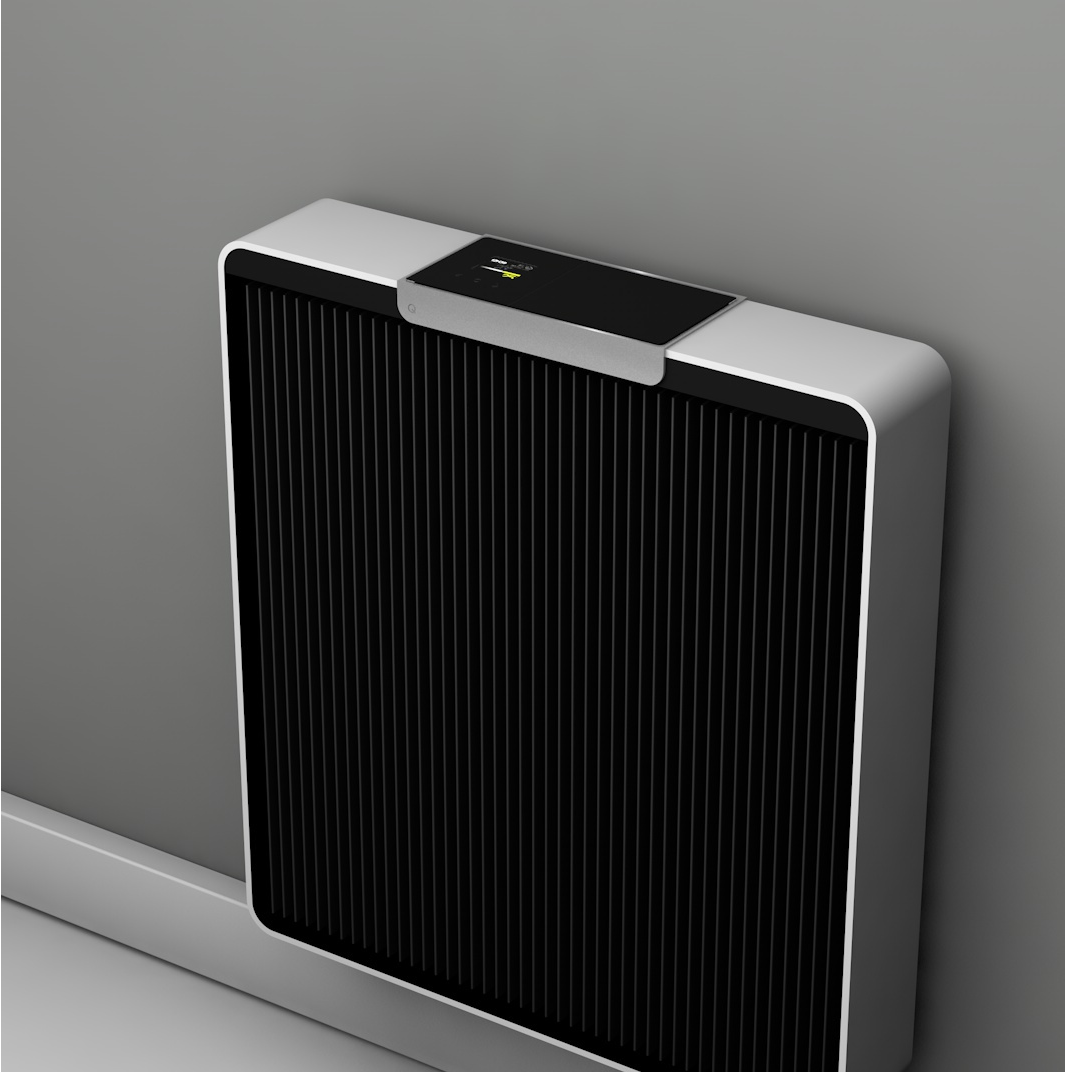
\includegraphics[width=4.2cm,height=4.2cm]{./Figures/rad.png}
            \caption{\scriptsize A Q.rad }
          \end{subfigure}
          \begin{subfigure}[b]{0.4\textwidth}
            \centering
            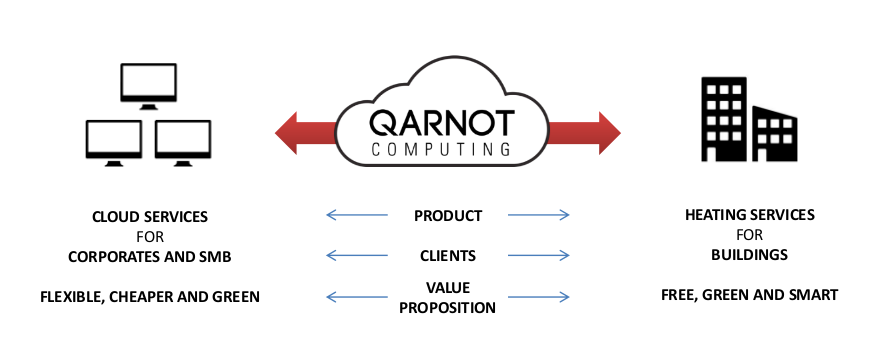
\includegraphics[width=10.7cm,height=4.2cm]{./Figures/model.png}
            \caption{\scriptsize The roles of the Q.ware }
          \end{subfigure}
	\caption{The Qarnot model}
	\label{fig:digital}
	\end{figure*}


Qarnot computing~\footnote{www.qarnot-computing.com} promotes a cloud computing model where heating, computing, 
storage and networking is provided from a 
single infrastructure. The latter consists in a network of geo-distributed servers deployed in homes, offices and buildings. 
The Qarnot model is based on two main products. The first is a new model of servers (Q.rads) in which the cooling system is replaced by a 
heat diffusion system, regulated by a thermostat. Each Q.rad (See Figure~\ref{fig:digital}) embeds several processors in addition to sensors 
related to humidity, $\mathrm{CO_2}$, presence etc. The second Qarnot product is a new middleware (Q.ware) for on-demand computing. Q.ware manages 
two types of requests: requests for the processing of cloud services  and requests for heating. Its goal is to deploy and 
adjust the run of cloud workload such as to meet the heat demand on Q.rads. For more details about the Qarnot model, we refer the interested 
reader to~\cite{DBLP:conf/europar/Ngoko16}. 

In the viewpoint of data or processes, the Qarnot model is very rich for in-situ machine learning. Indeed, in the data viewpoint, 
its sensing capacities can be used to create local datasets for any machine problem to solve at the scale of a home or building. 
For this the Qarnot platform supports a data service (QaIoT) that collects sensory data in Q.rads 
and make them available to programs designed for Q.rads. 
In the viewpoint of processes, the distributed learning processes can be performed in the home or building for which we want to 
build a learning system. For this, the Qarnot platform includes a software development kit (SDK) for building local orchestrations 
of processes in homes, buildings or cities.
The global objective of this paper is to show that with these two tools, 
complex in-situ machine learning workflows could be developed for smart-homes and buildings. For this, we focus on the resolution 
a problem that is interesting to address with in-situ learning: the construction of alarm sound classifiers. 
The interest in this problem comes from the fact that the behavior of an alarm sound classifier will be related to the background noises that 
it was trained with. Thus, depending on the environment in which we are, it is important to have the right background noises.

Our paper makes three important contributions. Firstly, we introduce a general orchestration system for implementing in-situ 
distributed learning frameworks and in particular, a solution for the alarm sounds detection, with the Qarnot SDK. 
The proposed orchestrator assumes an upper level abstraction close to the one used in GraphLab~\cite{Low:2012:DGF:2212351.2212354} (data model 
and update functions) and the concept of {\it Processors} used in the \texttt{madmom} library \cite{DBLP:journals/corr/BockKSKW16}. However, the abstraction is adjusted and adapted to fit with the object oriented interface 
of the Qarnot SDK. 
The alarm detection framework we use for validating the orchestrator is based on energy, spectral and Mel-frequency cepstral features~\cite{Davis:1990:CPR:108235.108239}, \cite{pyAudioAnalysis}
and a Pareto-selection method for choosing the best classifier from several techniques. % ATTENTION ICI : LES TECHNIQUES SONT EVALUEES SEPAREMENT DONC C'EST PAS VRAIMENT CA
The techniques include: the support vector machine, the logistic regression and the K-Nearest Neighbour. Our second contribution is to propose a possible parallel 
implementation for training the alarm framework based on the orchestrator we proposed. Finally, we explore this implementation and evaluate its accuracy, 
false and true positive rate and runtime performance. We compare two different types of work processing : a work-sharing-like in which the work is divided between the available nodes and a work-stealing-like in which the Q.ware scheduler runs an instance when nodes are available. This evaluation clearly states how we can decide on the most appropriate 
implementation. 

The remainder of the paper is organized as follows. In Section~\ref{Related}, we present the related works. 
In Section~\ref{Framework}, we discuss of the acoustic alarm detection framework that we consider. In Section~\ref{Model}, we describe 
the key services that the Qarnot platform offers for in-situ machine learning. In Section~\ref{Orchestrator}, we explain 
how we implement the training process of the framework that we introduced. A performance evaluation is done in 
Section~\ref{Proof-of-concept} and we conclude in Section~\ref{Conclusion}.

\section{Related work} \label{Related}


Our contribution is to put into perpective with the recent advances that led to the profusion of tools for parallel 
machine learning. Our work is also related to prior contributions in machine learning for acoustic alarm detection. 

Regarding recent parallel machine learning tools, we propose to distinguish between three main trends. 
The first trend includes the development of orchestrators for Big Data systems that are based on Hadoop~\footnote{http://hadoop.apache.org/}, Spark~\cite{Zaharia:2010:SCC:1863103.1863113} or related systems. 
In these solutions, the parallelism is generally formulated within the Map-reduce paradigm~\cite{DBLP:journals/cacm/DeanG10}. 
In the second trend, the restriction of the Map-reduce paradim are overcomed in using more general graph-based abstractions like 
the DAGs. Here, we are thinking to solutions that are related to 
the distributed GraphLab~\cite{Low:2012:DGF:2212351.2212354}.  Finally the last trend is related to the development of parallel 
systems for the the implementation of deep learning algorithms. Here, the key novelty is to exploit the parallelism at the GPU 
level~\cite{Raina:2009:LDU:1553374.1553486}.
Differently to these solutions, our proposition is neither based on Map-reduce, nor on GPUs. As already said, the orchestor we introduce 
is based on an upper layer abstraction close to the one we can find in GraphLab. However, our conceptualization manipulates object 
oriented concepts of the Qarnot SDK. In addition, our solution is specially designed for in-situ learning. 


The field of supervised machine learning for audio classification (that includes alarm sound detection) is well-established. There is a 
large consensus on the class of features that are meaningful in this context~\cite{Mckinney03featuresfor,DBLP:journals/taslp/JoderER09} 
and some classification 
methods like the logistic regression has been successfully applied in several cases. It was also showed 
that for sound detection systems to work in the real-world, it is important that the classifiers be trained with 
background noises that are representative of the environment in which the classifiers will operate~\cite{DBLP:conf/icassp/SalamonB15}. 
In other words, {\it in-situ} and context-aware learning is welcome on the problem. 

On this point, the work of Diane Watson et al.~\cite{watson_-situ_2012} shows that music recommender system can be improved if we 
account on the context in which the listener is. There are also several works like the one of Chu et al.~\cite{Chu:2009:ESR:1650051.1650059} 
that focus on the classification of audio environments. The work that we found closely related to ours is the Auditeur system~\cite{Nirjon:2013:AMS:2462456.2464446}. The system proposes a context-aware solution for acoustic events detection on smartphones. 
The Auditeur system is composed of: a phone client that captures, processes and can run a {\it classification plan} and a cloud 
service that based on audio and contextual information sent by a phone could generate an appropriate classification plan to be 
followed at the smartphone level. We did not investigate whether or not the workflow we propose could be applied 
to any acoustic event. But the main difference between our work and Auditeur is that we propose to collect and process 
data in a same environment. It is obvious to notice that such a solution is more interesting for real-time and security.



\section{Training framework for alarm sound detection } \label{Framework}

\subsection{General problem}

We assume a home with a fire-alarm and a set of Q.rads. Each Q.rad embeds two microphones and can record the input audio 
stream. We also assume that when recorded, the input stream is discretized into blocks of $T$ seconds that are written into a 
wav file. {\it The goal is to build  a detection system that given any wav file of $T$ seconds could state whether or not it contains 
an alarm sound}.

The system to build has $3$ subsystems: a data collection system, a training system and a decision system. 
The data collection system creates the dataset of wav files that will be used for training and validation. 
From the training dataset, the training system is able to generate the subset of dominant classifiers in considering 
the SVM, logistic regression and KNN techniques. Assuming we have classifiers that are trained for each input audio, 
the decision system states whether or not the audio contains a fire-alarm sound.

Our paper will mainly focus on the training system. However, we will shortly discuss of the data collection system in order 
to explain how we create training dataset in-situ.


\subsection{Data collection}

The challenging question here is to make sure that the data used for building the classifiers are representative of the environment 
in which the Q.rads are. For this, we propose to consider two main approaches. The first is to interact with the user in the 
home in order to record audio that includes an alarm sound and those that do not. In this way, the data collection and training systems 
could be seen as a {\it machine teaching system}. In this philosophy, let us notice that the expertise and level of cooperation 
of the user will decide on the quality of the generated classifiers. 
The second approach (that we will prefer) consists of the automatic generation of the dataset. 
For this, we suppose that we have a basis of alarm sounds that are the one we want to recognize. We also assume a basis of significative 
sounds like a baby cry or a music. In these audio records (alarm and significative sounds), there is no background 
noises. The goal of the data collection system is to create from this basis two datasets for training and evaluation where 
the background noises of the environment is introduced. This is summarized in Figure~\ref{fig:gen}. 
A challenge at this stage is to fix some programmability rules for recording 
background noises. We must also decide on the date at which we consider that a set of classifiers could be generated for exploitation. 
But due to space restriction, we will not discuss these details in this paper. However we will explain in Section~\ref{Model}, the 
system architecture that Qarnot proposes for in-situ data collection and processing.


	\begin{figure}[hbtp]
	\begin{center}
	%\fbox{
	% Graphic for TeX using PGF
% Title: /home/ngoko/Papiers/ParLearning2017/Figures/Aggregation.dia
% Creator: Dia v0.97.3
% CreationDate: Mon Dec 19 14:44:13 2016
% For: ngoko
% \usepackage{tikz}
% The following commands are not supported in PSTricks at present
% We define them conditionally, so when they are implemented,
% this pgf file will use them.
\ifx\du\undefined
  \newlength{\du}
\fi
\setlength{\du}{15\unitlength}
\begin{tikzpicture}
\pgftransformxscale{.52000000}
\pgftransformyscale{-.5200000}
\definecolor{dialinecolor}{rgb}{0.000000, 0.000000, 0.000000}
\pgfsetstrokecolor{dialinecolor}
\definecolor{dialinecolor}{rgb}{1.000000, 1.000000, 1.000000}
\pgfsetfillcolor{dialinecolor}
\pgfsetlinewidth{0.100000\du}
\pgfsetdash{}{0pt}
\pgfsetdash{}{0pt}
\pgfsetbuttcap
\pgfsetmiterjoin
\pgfsetlinewidth{0.100000\du}
\pgfsetbuttcap
\pgfsetmiterjoin
\pgfsetdash{}{0pt}
\definecolor{dialinecolor}{rgb}{1.000000, 1.000000, 1.000000}
\pgfsetfillcolor{dialinecolor}
\fill (23.700000\du,-133.100000\du)--(24.700000\du,-133.100000\du)--(24.700000\du,-132.600000\du)--(25.200000\du,-132.600000\du)--(25.200000\du,-131.100000\du)--(23.700000\du,-131.100000\du)--cycle;
\definecolor{dialinecolor}{rgb}{0.000000, 0.000000, 0.000000}
\pgfsetstrokecolor{dialinecolor}
\draw (23.700000\du,-133.100000\du)--(24.700000\du,-133.100000\du)--(24.700000\du,-132.600000\du)--(25.200000\du,-132.600000\du)--(25.200000\du,-131.100000\du)--(23.700000\du,-131.100000\du)--cycle;
\pgfsetlinewidth{0.010000\du}
\pgfsetbuttcap
\pgfsetmiterjoin
\pgfsetdash{}{0pt}
\definecolor{dialinecolor}{rgb}{0.000000, 0.000000, 0.000000}
\pgfsetstrokecolor{dialinecolor}
\draw (23.700000\du,-133.100000\du)--(24.700000\du,-133.100000\du)--(24.700000\du,-132.600000\du)--(25.200000\du,-132.600000\du)--(25.200000\du,-131.100000\du)--(23.700000\du,-131.100000\du)--cycle;
\pgfsetlinewidth{0.100000\du}
\pgfsetbuttcap
\pgfsetmiterjoin
\pgfsetdash{}{0pt}
\definecolor{dialinecolor}{rgb}{1.000000, 1.000000, 1.000000}
\pgfsetfillcolor{dialinecolor}
\fill (24.700000\du,-133.100000\du)--(25.200000\du,-132.600000\du)--(24.700000\du,-132.600000\du)--cycle;
\definecolor{dialinecolor}{rgb}{0.000000, 0.000000, 0.000000}
\pgfsetstrokecolor{dialinecolor}
\draw (24.700000\du,-133.100000\du)--(25.200000\du,-132.600000\du)--(24.700000\du,-132.600000\du)--cycle;
\pgfsetlinewidth{0.010000\du}
\pgfsetbuttcap
\pgfsetmiterjoin
\pgfsetdash{}{0pt}
\definecolor{dialinecolor}{rgb}{0.000000, 0.000000, 0.000000}
\pgfsetstrokecolor{dialinecolor}
\draw (24.700000\du,-133.100000\du)--(25.200000\du,-132.600000\du)--(24.700000\du,-132.600000\du)--cycle;
% setfont left to latex
\definecolor{dialinecolor}{rgb}{0.000000, 0.000000, 0.000000}
\pgfsetstrokecolor{dialinecolor}
\node at (24.450000\du,-130.250000\du){\small Alarm sounds};
\pgfsetlinewidth{0.100000\du}
\pgfsetdash{}{0pt}
\pgfsetdash{}{0pt}
\pgfsetbuttcap
\pgfsetmiterjoin
\pgfsetlinewidth{0.100000\du}
\pgfsetbuttcap
\pgfsetmiterjoin
\pgfsetdash{}{0pt}
\definecolor{dialinecolor}{rgb}{1.000000, 1.000000, 1.000000}
\pgfsetfillcolor{dialinecolor}
\fill (22.537750\du,-123.450789\du)--(23.809250\du,-123.450789\du)--(23.809250\du,-122.815039\du)--(24.445000\du,-122.815039\du)--(24.445000\du,-120.907789\du)--(22.537750\du,-120.907789\du)--cycle;
\definecolor{dialinecolor}{rgb}{0.000000, 0.000000, 0.000000}
\pgfsetstrokecolor{dialinecolor}
\draw (22.537750\du,-123.450789\du)--(23.809250\du,-123.450789\du)--(23.809250\du,-122.815039\du)--(24.445000\du,-122.815039\du)--(24.445000\du,-120.907789\du)--(22.537750\du,-120.907789\du)--cycle;
\pgfsetlinewidth{0.010000\du}
\pgfsetbuttcap
\pgfsetmiterjoin
\pgfsetdash{}{0pt}
\definecolor{dialinecolor}{rgb}{0.000000, 0.000000, 0.000000}
\pgfsetstrokecolor{dialinecolor}
\draw (22.537750\du,-123.450789\du)--(23.809250\du,-123.450789\du)--(23.809250\du,-122.815039\du)--(24.445000\du,-122.815039\du)--(24.445000\du,-120.907789\du)--(22.537750\du,-120.907789\du)--cycle;
\pgfsetlinewidth{0.100000\du}
\pgfsetbuttcap
\pgfsetmiterjoin
\pgfsetdash{}{0pt}
\definecolor{dialinecolor}{rgb}{1.000000, 1.000000, 1.000000}
\pgfsetfillcolor{dialinecolor}
\fill (23.809250\du,-123.450789\du)--(24.445000\du,-122.815039\du)--(23.809250\du,-122.815039\du)--cycle;
\definecolor{dialinecolor}{rgb}{0.000000, 0.000000, 0.000000}
\pgfsetstrokecolor{dialinecolor}
\draw (23.809250\du,-123.450789\du)--(24.445000\du,-122.815039\du)--(23.809250\du,-122.815039\du)--cycle;
\pgfsetlinewidth{0.010000\du}
\pgfsetbuttcap
\pgfsetmiterjoin
\pgfsetdash{}{0pt}
\definecolor{dialinecolor}{rgb}{0.000000, 0.000000, 0.000000}
\pgfsetstrokecolor{dialinecolor}
\draw (23.809250\du,-123.450789\du)--(24.445000\du,-122.815039\du)--(23.809250\du,-122.815039\du)--cycle;
% setfont left to latex
\definecolor{dialinecolor}{rgb}{0.000000, 0.000000, 0.000000}
\pgfsetstrokecolor{dialinecolor}
\node at (23.491375\du,-119.989914\du){\small Background noises};
\pgfsetlinewidth{0.100000\du}
\pgfsetdash{}{0pt}
\pgfsetdash{}{0pt}
\pgfsetbuttcap
\pgfsetmiterjoin
\pgfsetlinewidth{0.100000\du}
\pgfsetbuttcap
\pgfsetmiterjoin
\pgfsetdash{}{0pt}
\definecolor{dialinecolor}{rgb}{1.000000, 1.000000, 1.000000}
\pgfsetfillcolor{dialinecolor}
\pgfpathmoveto{\pgfpoint{30.987353\du}{-127.700000\du}}
\pgfpathcurveto{\pgfpoint{31.483824\du}{-127.700000\du}}{\pgfpoint{33.966176\du}{-127.700000\du}}{\pgfpoint{34.462647\du}{-127.700000\du}}
\pgfpathcurveto{\pgfpoint{34.959118\du}{-127.700000\du}}{\pgfpoint{34.959118\du}{-127.700000\du}}{\pgfpoint{34.959118\du}{-127.366667\du}}
\pgfpathcurveto{\pgfpoint{34.959118\du}{-127.033333\du}}{\pgfpoint{34.959118\du}{-126.366667\du}}{\pgfpoint{34.959118\du}{-126.033333\du}}
\pgfpathcurveto{\pgfpoint{34.959118\du}{-125.700000\du}}{\pgfpoint{34.959118\du}{-125.700000\du}}{\pgfpoint{34.462647\du}{-125.700000\du}}
\pgfpathcurveto{\pgfpoint{33.966176\du}{-125.700000\du}}{\pgfpoint{31.483824\du}{-125.700000\du}}{\pgfpoint{30.987353\du}{-125.700000\du}}
\pgfpathcurveto{\pgfpoint{30.490882\du}{-125.700000\du}}{\pgfpoint{30.490882\du}{-125.700000\du}}{\pgfpoint{30.490882\du}{-126.033333\du}}
\pgfpathcurveto{\pgfpoint{30.490882\du}{-126.366667\du}}{\pgfpoint{30.490882\du}{-127.033333\du}}{\pgfpoint{30.490882\du}{-127.366667\du}}
\pgfpathcurveto{\pgfpoint{30.490882\du}{-127.700000\du}}{\pgfpoint{30.490882\du}{-127.700000\du}}{\pgfpoint{30.987353\du}{-127.700000\du}}
\pgfusepath{fill}
\definecolor{dialinecolor}{rgb}{0.000000, 0.000000, 0.000000}
\pgfsetstrokecolor{dialinecolor}
\pgfpathmoveto{\pgfpoint{30.987353\du}{-127.700000\du}}
\pgfpathcurveto{\pgfpoint{31.483824\du}{-127.700000\du}}{\pgfpoint{33.966176\du}{-127.700000\du}}{\pgfpoint{34.462647\du}{-127.700000\du}}
\pgfpathcurveto{\pgfpoint{34.959118\du}{-127.700000\du}}{\pgfpoint{34.959118\du}{-127.700000\du}}{\pgfpoint{34.959118\du}{-127.366667\du}}
\pgfpathcurveto{\pgfpoint{34.959118\du}{-127.033333\du}}{\pgfpoint{34.959118\du}{-126.366667\du}}{\pgfpoint{34.959118\du}{-126.033333\du}}
\pgfpathcurveto{\pgfpoint{34.959118\du}{-125.700000\du}}{\pgfpoint{34.959118\du}{-125.700000\du}}{\pgfpoint{34.462647\du}{-125.700000\du}}
\pgfpathcurveto{\pgfpoint{33.966176\du}{-125.700000\du}}{\pgfpoint{31.483824\du}{-125.700000\du}}{\pgfpoint{30.987353\du}{-125.700000\du}}
\pgfpathcurveto{\pgfpoint{30.490882\du}{-125.700000\du}}{\pgfpoint{30.490882\du}{-125.700000\du}}{\pgfpoint{30.490882\du}{-126.033333\du}}
\pgfpathcurveto{\pgfpoint{30.490882\du}{-126.366667\du}}{\pgfpoint{30.490882\du}{-127.033333\du}}{\pgfpoint{30.490882\du}{-127.366667\du}}
\pgfpathcurveto{\pgfpoint{30.490882\du}{-127.700000\du}}{\pgfpoint{30.490882\du}{-127.700000\du}}{\pgfpoint{30.987353\du}{-127.700000\du}}
\pgfusepath{stroke}
\pgfsetlinewidth{0.010000\du}
\pgfsetbuttcap
\pgfsetmiterjoin
\pgfsetdash{}{0pt}
\definecolor{dialinecolor}{rgb}{0.000000, 0.000000, 0.000000}
\pgfsetstrokecolor{dialinecolor}
\pgfpathmoveto{\pgfpoint{30.987353\du}{-127.700000\du}}
\pgfpathcurveto{\pgfpoint{31.483824\du}{-127.700000\du}}{\pgfpoint{33.966176\du}{-127.700000\du}}{\pgfpoint{34.462647\du}{-127.700000\du}}
\pgfpathcurveto{\pgfpoint{34.959118\du}{-127.700000\du}}{\pgfpoint{34.959118\du}{-127.700000\du}}{\pgfpoint{34.959118\du}{-127.366667\du}}
\pgfpathcurveto{\pgfpoint{34.959118\du}{-127.033333\du}}{\pgfpoint{34.959118\du}{-126.366667\du}}{\pgfpoint{34.959118\du}{-126.033333\du}}
\pgfpathcurveto{\pgfpoint{34.959118\du}{-125.700000\du}}{\pgfpoint{34.959118\du}{-125.700000\du}}{\pgfpoint{34.462647\du}{-125.700000\du}}
\pgfpathcurveto{\pgfpoint{33.966176\du}{-125.700000\du}}{\pgfpoint{31.483824\du}{-125.700000\du}}{\pgfpoint{30.987353\du}{-125.700000\du}}
\pgfpathcurveto{\pgfpoint{30.490882\du}{-125.700000\du}}{\pgfpoint{30.490882\du}{-125.700000\du}}{\pgfpoint{30.490882\du}{-126.033333\du}}
\pgfpathcurveto{\pgfpoint{30.490882\du}{-126.366667\du}}{\pgfpoint{30.490882\du}{-127.033333\du}}{\pgfpoint{30.490882\du}{-127.366667\du}}
\pgfpathcurveto{\pgfpoint{30.490882\du}{-127.700000\du}}{\pgfpoint{30.490882\du}{-127.700000\du}}{\pgfpoint{30.987353\du}{-127.700000\du}}
\pgfusepath{stroke}
\pgfsetbuttcap
\pgfsetmiterjoin
\pgfsetdash{}{0pt}
\definecolor{dialinecolor}{rgb}{0.000000, 0.000000, 0.000000}
\pgfsetstrokecolor{dialinecolor}
\draw (30.987353\du,-125.700000\du)--(34.462647\du,-125.700000\du);
\pgfsetbuttcap
\pgfsetmiterjoin
\pgfsetdash{}{0pt}
\definecolor{dialinecolor}{rgb}{0.000000, 0.000000, 0.000000}
\pgfsetstrokecolor{dialinecolor}
\draw (34.959118\du,-127.366667\du)--(34.959118\du,-126.033333\du);
\pgfsetbuttcap
\pgfsetmiterjoin
\pgfsetdash{}{0pt}
\definecolor{dialinecolor}{rgb}{0.000000, 0.000000, 0.000000}
\pgfsetstrokecolor{dialinecolor}
\draw (30.490882\du,-127.366667\du)--(30.490882\du,-126.033333\du);
\pgfsetbuttcap
\pgfsetmiterjoin
\pgfsetdash{}{0pt}
\definecolor{dialinecolor}{rgb}{0.000000, 0.000000, 0.000000}
\pgfsetstrokecolor{dialinecolor}
\draw (30.987353\du,-127.700000\du)--(34.462647\du,-127.700000\du);
% setfont left to latex
\definecolor{dialinecolor}{rgb}{0.000000, 0.000000, 0.000000}
\pgfsetstrokecolor{dialinecolor}
\node at (32.725000\du,-126.60000\du){\small Mixer};
\pgfsetlinewidth{0.100000\du}
\pgfsetdash{}{0pt}
\pgfsetdash{}{0pt}
\pgfsetbuttcap
\pgfsetmiterjoin
\pgfsetlinewidth{0.100000\du}
\pgfsetbuttcap
\pgfsetmiterjoin
\pgfsetdash{}{0pt}
\definecolor{dialinecolor}{rgb}{1.000000, 1.000000, 1.000000}
\pgfsetfillcolor{dialinecolor}
\fill (22.600000\du,-128.100000\du)--(23.600000\du,-128.100000\du)--(23.600000\du,-127.600000\du)--(24.100000\du,-127.600000\du)--(24.100000\du,-126.100000\du)--(22.600000\du,-126.100000\du)--cycle;
\definecolor{dialinecolor}{rgb}{0.000000, 0.000000, 0.000000}
\pgfsetstrokecolor{dialinecolor}
\draw (22.600000\du,-128.100000\du)--(23.600000\du,-128.100000\du)--(23.600000\du,-127.600000\du)--(24.100000\du,-127.600000\du)--(24.100000\du,-126.100000\du)--(22.600000\du,-126.100000\du)--cycle;
\pgfsetlinewidth{0.010000\du}
\pgfsetbuttcap
\pgfsetmiterjoin
\pgfsetdash{}{0pt}
\definecolor{dialinecolor}{rgb}{0.000000, 0.000000, 0.000000}
\pgfsetstrokecolor{dialinecolor}
\draw (22.600000\du,-128.100000\du)--(23.600000\du,-128.100000\du)--(23.600000\du,-127.600000\du)--(24.100000\du,-127.600000\du)--(24.100000\du,-126.100000\du)--(22.600000\du,-126.100000\du)--cycle;
\pgfsetlinewidth{0.100000\du}
\pgfsetbuttcap
\pgfsetmiterjoin
\pgfsetdash{}{0pt}
\definecolor{dialinecolor}{rgb}{1.000000, 1.000000, 1.000000}
\pgfsetfillcolor{dialinecolor}
\fill (23.600000\du,-128.100000\du)--(24.100000\du,-127.600000\du)--(23.600000\du,-127.600000\du)--cycle;
\definecolor{dialinecolor}{rgb}{0.000000, 0.000000, 0.000000}
\pgfsetstrokecolor{dialinecolor}
\draw (23.600000\du,-128.100000\du)--(24.100000\du,-127.600000\du)--(23.600000\du,-127.600000\du)--cycle;
\pgfsetlinewidth{0.010000\du}
\pgfsetbuttcap
\pgfsetmiterjoin
\pgfsetdash{}{0pt}
\definecolor{dialinecolor}{rgb}{0.000000, 0.000000, 0.000000}
\pgfsetstrokecolor{dialinecolor}
\draw (23.600000\du,-128.100000\du)--(24.100000\du,-127.600000\du)--(23.600000\du,-127.600000\du)--cycle;
% setfont left to latex
\definecolor{dialinecolor}{rgb}{0.000000, 0.000000, 0.000000}
\pgfsetstrokecolor{dialinecolor}
\node at (23.350000\du,-125.250000\du){\small Significative sounds};
% setfont left to latex
\definecolor{dialinecolor}{rgb}{0.000000, 0.000000, 0.000000}
\pgfsetstrokecolor{dialinecolor}
\node[anchor=west] at (42.700000\du,-131.250000\du){};
\pgfsetlinewidth{0.100000\du}
\pgfsetdash{}{0pt}
\pgfsetdash{}{0pt}
\pgfsetbuttcap
\pgfsetmiterjoin
\pgfsetlinewidth{0.100000\du}
\pgfsetbuttcap
\pgfsetmiterjoin
\pgfsetdash{}{0pt}
\definecolor{dialinecolor}{rgb}{1.000000, 1.000000, 1.000000}
\pgfsetfillcolor{dialinecolor}
\fill (41.595000\du,-133.329289\du)--(42.595000\du,-133.329289\du)--(42.595000\du,-132.829289\du)--(43.095000\du,-132.829289\du)--(43.095000\du,-131.329289\du)--(41.595000\du,-131.329289\du)--cycle;
\definecolor{dialinecolor}{rgb}{0.000000, 0.000000, 0.000000}
\pgfsetstrokecolor{dialinecolor}
\draw (41.595000\du,-133.329289\du)--(42.595000\du,-133.329289\du)--(42.595000\du,-132.829289\du)--(43.095000\du,-132.829289\du)--(43.095000\du,-131.329289\du)--(41.595000\du,-131.329289\du)--cycle;
\pgfsetlinewidth{0.010000\du}
\pgfsetbuttcap
\pgfsetmiterjoin
\pgfsetdash{}{0pt}
\definecolor{dialinecolor}{rgb}{0.000000, 0.000000, 0.000000}
\pgfsetstrokecolor{dialinecolor}
\draw (41.595000\du,-133.329289\du)--(42.595000\du,-133.329289\du)--(42.595000\du,-132.829289\du)--(43.095000\du,-132.829289\du)--(43.095000\du,-131.329289\du)--(41.595000\du,-131.329289\du)--cycle;
\pgfsetlinewidth{0.100000\du}
\pgfsetbuttcap
\pgfsetmiterjoin
\pgfsetdash{}{0pt}
\definecolor{dialinecolor}{rgb}{1.000000, 1.000000, 1.000000}
\pgfsetfillcolor{dialinecolor}
\fill (42.595000\du,-133.329289\du)--(43.095000\du,-132.829289\du)--(42.595000\du,-132.829289\du)--cycle;
\definecolor{dialinecolor}{rgb}{0.000000, 0.000000, 0.000000}
\pgfsetstrokecolor{dialinecolor}
\draw (42.595000\du,-133.329289\du)--(43.095000\du,-132.829289\du)--(42.595000\du,-132.829289\du)--cycle;
\pgfsetlinewidth{0.010000\du}
\pgfsetbuttcap
\pgfsetmiterjoin
\pgfsetdash{}{0pt}
\definecolor{dialinecolor}{rgb}{0.000000, 0.000000, 0.000000}
\pgfsetstrokecolor{dialinecolor}
\draw (42.595000\du,-133.329289\du)--(43.095000\du,-132.829289\du)--(42.595000\du,-132.829289\du)--cycle;
% setfont left to latex
\definecolor{dialinecolor}{rgb}{0.000000, 0.000000, 0.000000}
\pgfsetstrokecolor{dialinecolor}
\node at (42.345000\du,-130.479289\du){\small Alarm+};
% setfont left to latex
\definecolor{dialinecolor}{rgb}{0.000000, 0.000000, 0.000000}
\pgfsetstrokecolor{dialinecolor}
\node at (42.345000\du,-129.679289\du){\small Background};
\pgfsetlinewidth{0.100000\du}
\pgfsetdash{}{0pt}
\pgfsetdash{}{0pt}
\pgfsetbuttcap
\pgfsetmiterjoin
\pgfsetlinewidth{0.100000\du}
\pgfsetbuttcap
\pgfsetmiterjoin
\pgfsetdash{}{0pt}
\definecolor{dialinecolor}{rgb}{1.000000, 1.000000, 1.000000}
\pgfsetfillcolor{dialinecolor}
\fill (41.525000\du,-127.679289\du)--(42.525000\du,-127.679289\du)--(42.525000\du,-127.179289\du)--(43.025000\du,-127.179289\du)--(43.025000\du,-125.679289\du)--(41.525000\du,-125.679289\du)--cycle;
\definecolor{dialinecolor}{rgb}{0.000000, 0.000000, 0.000000}
\pgfsetstrokecolor{dialinecolor}
\draw (41.525000\du,-127.679289\du)--(42.525000\du,-127.679289\du)--(42.525000\du,-127.179289\du)--(43.025000\du,-127.179289\du)--(43.025000\du,-125.679289\du)--(41.525000\du,-125.679289\du)--cycle;
\pgfsetlinewidth{0.010000\du}
\pgfsetbuttcap
\pgfsetmiterjoin
\pgfsetdash{}{0pt}
\definecolor{dialinecolor}{rgb}{0.000000, 0.000000, 0.000000}
\pgfsetstrokecolor{dialinecolor}
\draw (41.525000\du,-127.679289\du)--(42.525000\du,-127.679289\du)--(42.525000\du,-127.179289\du)--(43.025000\du,-127.179289\du)--(43.025000\du,-125.679289\du)--(41.525000\du,-125.679289\du)--cycle;
\pgfsetlinewidth{0.100000\du}
\pgfsetbuttcap
\pgfsetmiterjoin
\pgfsetdash{}{0pt}
\definecolor{dialinecolor}{rgb}{1.000000, 1.000000, 1.000000}
\pgfsetfillcolor{dialinecolor}
\fill (42.525000\du,-127.679289\du)--(43.025000\du,-127.179289\du)--(42.525000\du,-127.179289\du)--cycle;
\definecolor{dialinecolor}{rgb}{0.000000, 0.000000, 0.000000}
\pgfsetstrokecolor{dialinecolor}
\draw (42.525000\du,-127.679289\du)--(43.025000\du,-127.179289\du)--(42.525000\du,-127.179289\du)--cycle;
\pgfsetlinewidth{0.010000\du}
\pgfsetbuttcap
\pgfsetmiterjoin
\pgfsetdash{}{0pt}
\definecolor{dialinecolor}{rgb}{0.000000, 0.000000, 0.000000}
\pgfsetstrokecolor{dialinecolor}
\draw (42.525000\du,-127.679289\du)--(43.025000\du,-127.179289\du)--(42.525000\du,-127.179289\du)--cycle;
% setfont left to latex
\definecolor{dialinecolor}{rgb}{0.000000, 0.000000, 0.000000}
\pgfsetstrokecolor{dialinecolor}
\node at (42.275000\du,-124.829289\du){\small Significative sounds+};
% setfont left to latex
\definecolor{dialinecolor}{rgb}{0.000000, 0.000000, 0.000000}
\pgfsetstrokecolor{dialinecolor}
\node at (42.275000\du,-124.029289\du){\small Background};
\pgfsetlinewidth{0.100000\du}
\pgfsetdash{}{0pt}
\pgfsetdash{}{0pt}
\pgfsetbuttcap
\pgfsetmiterjoin
\pgfsetlinewidth{0.100000\du}
\pgfsetbuttcap
\pgfsetmiterjoin
\pgfsetdash{}{0pt}
\definecolor{dialinecolor}{rgb}{1.000000, 1.000000, 1.000000}
\pgfsetfillcolor{dialinecolor}
\fill (41.390125\du,-122.479289\du)--(42.661625\du,-122.479289\du)--(42.661625\du,-121.843539\du)--(43.297375\du,-121.843539\du)--(43.297375\du,-119.936289\du)--(41.390125\du,-119.936289\du)--cycle;
\definecolor{dialinecolor}{rgb}{0.000000, 0.000000, 0.000000}
\pgfsetstrokecolor{dialinecolor}
\draw (41.390125\du,-122.479289\du)--(42.661625\du,-122.479289\du)--(42.661625\du,-121.843539\du)--(43.297375\du,-121.843539\du)--(43.297375\du,-119.936289\du)--(41.390125\du,-119.936289\du)--cycle;
\pgfsetlinewidth{0.010000\du}
\pgfsetbuttcap
\pgfsetmiterjoin
\pgfsetdash{}{0pt}
\definecolor{dialinecolor}{rgb}{0.000000, 0.000000, 0.000000}
\pgfsetstrokecolor{dialinecolor}
\draw (41.390125\du,-122.479289\du)--(42.661625\du,-122.479289\du)--(42.661625\du,-121.843539\du)--(43.297375\du,-121.843539\du)--(43.297375\du,-119.936289\du)--(41.390125\du,-119.936289\du)--cycle;
\pgfsetlinewidth{0.100000\du}
\pgfsetbuttcap
\pgfsetmiterjoin
\pgfsetdash{}{0pt}
\definecolor{dialinecolor}{rgb}{1.000000, 1.000000, 1.000000}
\pgfsetfillcolor{dialinecolor}
\fill (42.661625\du,-122.479289\du)--(43.297375\du,-121.843539\du)--(42.661625\du,-121.843539\du)--cycle;
\definecolor{dialinecolor}{rgb}{0.000000, 0.000000, 0.000000}
\pgfsetstrokecolor{dialinecolor}
\draw (42.661625\du,-122.479289\du)--(43.297375\du,-121.843539\du)--(42.661625\du,-121.843539\du)--cycle;
\pgfsetlinewidth{0.010000\du}
\pgfsetbuttcap
\pgfsetmiterjoin
\pgfsetdash{}{0pt}
\definecolor{dialinecolor}{rgb}{0.000000, 0.000000, 0.000000}
\pgfsetstrokecolor{dialinecolor}
\draw (42.661625\du,-122.479289\du)--(43.297375\du,-121.843539\du)--(42.661625\du,-121.843539\du)--cycle;
% setfont left to latex
\definecolor{dialinecolor}{rgb}{0.000000, 0.000000, 0.000000}
\pgfsetstrokecolor{dialinecolor}
\node at (42.343750\du,-119.018414\du){\small Background noises};
\pgfsetlinewidth{0.100000\du}
\pgfsetdash{}{0pt}
\pgfsetdash{}{0pt}
\pgfsetbuttcap
{
\definecolor{dialinecolor}{rgb}{0.000000, 0.000000, 0.000000}
\pgfsetfillcolor{dialinecolor}
% was here!!!
\pgfsetarrowsend{stealth}
\definecolor{dialinecolor}{rgb}{0.000000, 0.000000, 0.000000}
\pgfsetstrokecolor{dialinecolor}
\draw (26.900000\du,-129.950000\du)--(30.490882\du,-127.366667\du);
}
\pgfsetlinewidth{0.100000\du}
\pgfsetdash{}{0pt}
\pgfsetdash{}{0pt}
\pgfsetbuttcap
{
\definecolor{dialinecolor}{rgb}{0.000000, 0.000000, 0.000000}
\pgfsetfillcolor{dialinecolor}
% was here!!!
\pgfsetarrowsend{stealth}
\definecolor{dialinecolor}{rgb}{0.000000, 0.000000, 0.000000}
\pgfsetstrokecolor{dialinecolor}
\draw (24.075000\du,-126.725000\du)--(30.490882\du,-126.700000\du);
}
\pgfsetlinewidth{0.100000\du}
\pgfsetdash{}{0pt}
\pgfsetdash{}{0pt}
\pgfsetbuttcap
{
\definecolor{dialinecolor}{rgb}{0.000000, 0.000000, 0.000000}
\pgfsetfillcolor{dialinecolor}
% was here!!!
\pgfsetarrowsend{stealth}
\definecolor{dialinecolor}{rgb}{0.000000, 0.000000, 0.000000}
\pgfsetstrokecolor{dialinecolor}
\draw (24.750000\du,-122.900000\du)--(30.490882\du,-126.033333\du);
}
\pgfsetlinewidth{0.100000\du}
\pgfsetdash{}{0pt}
\pgfsetdash{}{0pt}
\pgfsetbuttcap
{
\definecolor{dialinecolor}{rgb}{0.000000, 0.000000, 0.000000}
\pgfsetfillcolor{dialinecolor}
% was here!!!
\pgfsetarrowsend{stealth}
\definecolor{dialinecolor}{rgb}{0.000000, 0.000000, 0.000000}
\pgfsetstrokecolor{dialinecolor}
\draw (34.959118\du,-127.366667\du)--(41.595000\du,-131.829289\du);
}
\pgfsetlinewidth{0.100000\du}
\pgfsetdash{}{0pt}
\pgfsetdash{}{0pt}
\pgfsetbuttcap
{
\definecolor{dialinecolor}{rgb}{0.000000, 0.000000, 0.000000}
\pgfsetfillcolor{dialinecolor}
% was here!!!
\pgfsetarrowsend{stealth}
\definecolor{dialinecolor}{rgb}{0.000000, 0.000000, 0.000000}
\pgfsetstrokecolor{dialinecolor}
\draw (34.959118\du,-126.700000\du)--(41.525000\du,-126.679289\du);
}
\pgfsetlinewidth{0.100000\du}
\pgfsetdash{}{0pt}
\pgfsetdash{}{0pt}
\pgfsetbuttcap
{
\definecolor{dialinecolor}{rgb}{0.000000, 0.000000, 0.000000}
\pgfsetfillcolor{dialinecolor}
% was here!!!
\pgfsetarrowsend{stealth}
\definecolor{dialinecolor}{rgb}{0.000000, 0.000000, 0.000000}
\pgfsetstrokecolor{dialinecolor}
\draw (34.959118\du,-126.033333\du)--(41.237500\du,-121.925000\du);
}
\end{tikzpicture}

	%}
	\caption{Automatic generation of the dataset: we mix alarm and significative sounds with the local background noises.}
	\label{fig:gen}
	\end{center}
	\end{figure}


\subsection{Training system}

In Figure~\ref{fig:training}, we illustrate the training framework we consider in our problem. The representation follows the 
BPMN notation (An empty lozenge is a join and a lozenge with a plus is a fork...). 

	\begin{figure*}[htbp]
	\centering
	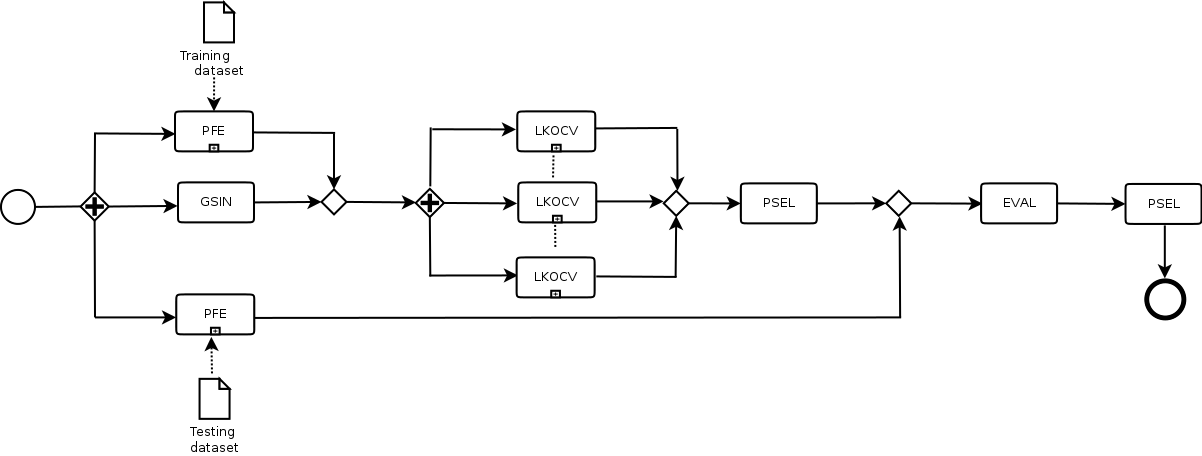
\includegraphics[width=13cm, height=5 cm]{./Figures/workflow.png}
	\caption{Training system}
	\label{fig:training}
	\end{figure*}

The framework is based on 5 activities and subprocesses that we discuss below.

\begin{itemize}

\item {\bf PFE:} Given a set of wav files, the goal here is to extract the acoustic features of the wav files. PFE is a subprocess 
consisting of a set of parallel activities where the acoustic features are separately computed from each dataset file. 
The features we used are the classical ones used in signal processing (Mel-frequency spectrum~\cite{Davis:1990:CPR:108235.108239}, 
energy etc.). Their complete list is defined in~\cite{pyAudioAnalysis}. 

\item {\bf GSIN:} The framework implements a grid search process whose goal is to find the best classifiers depending on the 
parameters we use. GSIN consists in the initialization of this grid search. The goal is to generate the possible configurations 
we will use in the search of the best classifiers. 

\item {\bf LKOCV:} Given an input configuration (generated in GSIN), this subprocess starts with the run of a 
time integration method whose goal is to refine the training features according to the input configuration. The idea is 
to aggregate the values of acoustic features in time such as to refine the quality of information they provide. The integration 
methods we used are defined in~\cite{DBLP:journals/taslp/JoderER09} (only taking the mean, the mean and variance and concatenating the features were implemented). With the refined features, the next activity in the subprocess consists in evaluating the classifier corresponding to the current configuration with a Leave-k-out cross-validation. Our learning techniques include: the SVM, logistic regression and KNN. 

\item {\bf PSEL:} From a list of classifiers whose False and True Positive rates (FPR, TPR) are defined (generated in LKOCV or EVAL), we select the ones that are in the Pareto front where we minimize the FPR and maximize the TPR.

\item {\bf EVAL:}  Assuming a list of classifiers and the input features of the testing dataset, we evaluate here the classifiers on the testing features. The TPR and FPR of each classifier are returned.

\end{itemize}

The proposed framework is parallel and distributed. In the next, we will discuss of the component of the Qarnot architecture for 
its implementation.

\section{Architecture and programming model} \label{Model}

In the viewpoint of data, the network of Q.rads at the scale of a city or building is a composition of clusters, each 
associated with a QaIoT server. A QaIoT server aggregates and manages the sensory data issued from the Q.rads to which it is 
connected. A program deployed on the a connected device (or a Q.rad) can get access to these data. For this purpose, 
it must first register to the QaIoT server in sending an Http request where it declines: the nature of the device (Q.rad, 
raspberry etc.), the Id of the device, the role it intends to play (e.g: access to the audio stream of the cluster). If the 
request is accepted a websocket communication will  be established between the device and QaIoT in order to distribute the data 
to service the data to the applicant program. Let us suppose that this communication can consist of servicing real-time data 
to the applicant program. An illustration is provided in Figure~\ref{fig:arch}(a). 
It is easy to notice that the mixer of Figure~\ref{fig:gen} can be implemented as an applicant program that request the audio streams  
related to a home and then {\it mixes} the data with a set of alarms and significant sounds.

In the processing viewpoint, the Qarnot SDK is based on three main concepts: the notion of task (referred to as {\it QTask}), 
the notion of disk ({\it QDisk}) and the docker image. A task is an object oriented abstraction that natively refers to a 
docker or a set of docker containers to deploy and run. A task is associated with a docker image defined in the 
parameter {\it constants["DOCKER\_REPO"]}. We can specify a set of input files for a task in defining a resource disk. 
The input disk is defined in the list parameter {\it resources}. A task has a name and can be composed by subtasks (or frames).  
In these cases, the run of each subtask will cause the deployment of a docker image. The process run by a task is defined in 
assigning a command line to the parameter {\it constants['DOCKER\_CMD']}. The execution will assume that the input files are available 
from the disks defined in {\it resources}, and will generate a result disk if the task produces files.


	\begin{figure*}[ht]
          \begin{subfigure}[b]{0.4\textwidth}
            \centering
            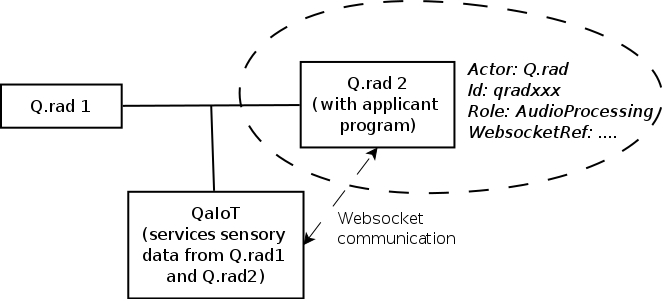
\includegraphics[scale=0.3]{./Figures/DataService.png}
            \caption{Data service}
          \end{subfigure}
          \begin{subfigure}[b]{0.6\textwidth}
            \centering
            \inputminted[baselinestretch=1.2, bgcolor=LightGray, fontsize=\scriptsize]{python}{sample.py}
            \caption{Example of scripts with the Qarnot SDK}
          \end{subfigure}
          \caption{Data service and Qarnot SDK example.} 
          \label{fig:arch}
	\end{figure*}

An example of script with the Qarnot SDK is proposed in Figure~\ref{fig:arch}(b). Finally, for in-situ learning, let us notice that 
in using the constants, of a task, we can constraint its execution to be done only on a Q.rad or a set of Q.rad.


\section{Orchestrating the alarm detection framework} \label{Orchestrator}
\subsection{The orchestrator}
The orchestration method implemented for the framework relies on 2 basic concepts (implemented in \texttt{python}): 
\begin{itemize}
\item \textbf{QWork:} This represents a work to be done during the workflow. QWorks correspond to boxes in a diagram. They have 2 main attributes : \texttt{name} which enables to differentiate the QWorks and \texttt{nextname} which enables to define the next QWork in the workflow. A QWork also has a \texttt{process} method which represents the work to do. To make it even simpler, QWork instances are callable which means that they can be used as any function. 
\item \textbf{QData:} This represents the inputs and outputs of QWorks. QData correspond to arrows in a diagram. A QData instance is a dictionary with 3 keys (it can be seen as a 3 columns table and we will keep this analogy for clarity): \texttt{data} (the actual data), \texttt{sender} (the name of the QWork which sends the data) and \texttt{receiver} (the name of the QWork which receives the data). 
\end{itemize}
These two concept work together as follows : let \texttt{w} be an instance of QWork and \texttt{d} and instance of QData. Running \texttt{w(d)} makes \texttt{w} look for its \texttt{name} in \texttt{d}'s \texttt{receiver} column and process the the corresponding row using the \texttt{process} method. In the \texttt{process} method, one can specify how to handle different \texttt{senders}.

Subclasses of QWork can then be defined to differentiate what is done locally and what is done in parallel using the Qarnot platform : 
\begin{itemize}
\item \textbf{QFunc:} a QFunc is a QWork which processes a particular function given when instantiating the class
\item \textbf{QTask:} a QTask is a QWork and a Task (from the qarnot SDK). The QTask class has two particularities : 
the first one is that its input must be a disk (which will be added it to the resources) or a serializable object (which will be put in a resource disk). This is done with a method called \texttt{add\_input\_to\_resources}. The second one is that there are two ways to run a QTask instance : \texttt{process} method (or calling the instance which is the same) which will submit the task and wait for it to be over, and the \texttt{submit} method which does not wait for the task to be over (which is useful for parallel tasks, see below). The output of a QTask is its results disk.
\end{itemize}
With these three tools (QData, QFunc, QTask) one could create basic parallel workflows composed of functions and tasks. To go a step further in the abstraction, we created two other subclasses of QWork that represent higher level concepts : 
\begin{itemize}
\item \textbf{QParallelWork:} A QParallelWork instance has a list of QWorks (except QTasks) and a list of QTasks and runs all of them in parallel using different threads (here QTasks and other QWorks were separated because we use the \texttt{submit} method for QTasks which does not exist in the others).
\item \textbf{QWorklow:} This is the highest concept since it represents the workflow itself. A QWorkflow task has a list of QWorks and runs them in a {\it greedy} way which means that it only runs a QWork when its needed inputs are available (i.e when the previous QWork in the list stops).
\end{itemize}
To sum up, there are 4 subclasses of QWork : QFunc for basic functions, QTasks for tasks, QParallelWork for multithreading and QWorkflow to combine them all. QData makes the link between them.

By combining all these concepts, complex workflows can be implemented. Note that a QWorkflows can be put in a QParallelWork to run multiple workflows simultaneously. 

Algorithms \ref{alg:Qwork}, \ref{alg:Qtask}, \ref{alg:Qparallel}, \ref{alg:Qworkflow} sum up in pseudo-code the ways these concepts handle a given input. A QWork will call its \texttt{process} method. A QFunc's \texttt{process} method calls the function. A QTask will add the inputs to its resources and submit the task to the Q.Ware scheduler. A QParallelWork will submit all QTasks and run all other QWorks in different threads and then wait for all of them to finish. A QWorkflow will run all its QWorks.

Note that all QWorks which are not QTasks are processed locally, where the global QWorkflow is running, and all QTasks are submited to the Q.Ware scheduler for parallel processing. Moreover, the QTasks can be constrained to run the Q.rads of a house, a building on several buildings. In-Situ machine learning can then be done by running the global QWorkflow on one Q.rad of the house and constraining the QTasks to all the house's Q.rads.

In all the algorithms presented, QWorks need a QData as input, therefore if one wants do create a QFunc with multiple input there are two ways :
\begin{itemize}
\item Get inputs as different QData rows then differentiate inputs according to the \texttt{sender} (see for example \texttt{f211} in figure \ref{fig:orch_ex})
\item Put a dictionary in the QData \texttt{data} column (see for example QCreateDisk below)
\end{itemize}

\begin{algorithm}[H]
\caption{QWork call method}
\label{alg:Qwork}
\begin{algorithmic}
\REQUIRE \texttt{d} a QData instance
\ENSURE returns \texttt{d} without my input, with my output
\STATE find my name in \texttt{d["receiver"]}, remove the corresponding rows from \texttt{d} and put them in \texttt{d'}
\STATE out $\leftarrow$ \texttt{process}(\texttt{d'})
\STATE add out to \texttt{d}
\RETURN \texttt{d}
\end{algorithmic}
\end{algorithm}

\begin{algorithm}[H]
\caption{QTask submit method}
\label{alg:Qtask}
\begin{algorithmic}
\REQUIRE \texttt{d} a QData instance
\ENSURE adds the input to resources and submits the task
\STATE find my name in \texttt{d["receiver"]}, remove the corresponding rows from \texttt{d} and put them in \texttt{d'}
\STATE \texttt{add\_input\_to\_resources}(\texttt{d'})
\STATE submit the task
\end{algorithmic}
\end{algorithm}

\begin{algorithm}
\caption{QParallelWork call method}
\label{alg:Qparallel}
\begin{algorithmic}
\REQUIRE \texttt{d} a QData instance
\ENSURE returns \texttt{d} without my QWorks and QTasks inputs and with the outputs
\FOR{\texttt{w} in my list of QWorks and my list of QTasks}
\STATE find \texttt{w.name} in \texttt{d["receiver"]}, remove the corresponding rows from \texttt{d} and put them in \texttt{d'}
\ENDFOR
\FOR{\texttt{w} in in my list of QWorks}
\STATE find \texttt{w.name} in \texttt{d'["receiver"]}, remove the corresponding rows from \texttt{d} and put them in \texttt{d'}
\STATE create a thread to run \texttt{w}($d''$)
\ENDFOR
\FOR{\texttt{t} in in my list of QTasks}
\STATE find \texttt{t.name} in \texttt{d'["receiver"]}, remove the corresponding rows from \texttt{d} and put them in \texttt{d'}
\STATE \texttt{t.add\_input\_to\_resources}(\texttt{d'})
\STATE \texttt{t.submit()}
\ENDFOR
\STATE wait for every thread and every task to end
\STATE add all outputs to \texttt{d}
\RETURN \texttt{d}
\end{algorithmic}
\end{algorithm}

\begin{algorithm}
\caption{QWorkflow process method}
\label{alg:Qworkflow}
\begin{algorithmic}
\REQUIRE \texttt{d} a QData instance
\ENSURE runs the Qworks sequentially
\STATE \texttt{in} $\leftarrow \texttt{d}$
\FOR{\texttt{w} in my list of QWorks}
\STATE \texttt{in} = \texttt{w}(\texttt{in})
\ENDFOR
\RETURN \texttt{in}
\end{algorithmic}
\end{algorithm}

In the next subsections, we present a simple example and an implementation of the framework using the orchestrator.
 
\subsection{A simple orchestration example}
We present here a simple example using the orchestration, the workflow consists in basic operations on numbers but shows how to use the different concepts to go from a diagram to the code. The diagram, the \texttt{python} code  and a part of the \texttt{stdout} are presented in figure \ref{fig:orch_ex}
\begin{figure*}[hbtp]
  \centering
  \begin{tabular}[c]{cc}
    \begin{subfigure}[b]{.55\textwidth}
      \inputminted[baselinestretch=1, bgcolor=LightGray,fontsize=\footnotesize]{python}{orchestration_example.py}
      \caption{Source code. The output is $13$}
    \end{subfigure}
    &
    \begin{tabular}[b]{c}
      \begin{subfigure}[t]{.5\textwidth}
      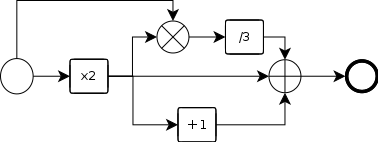
\includegraphics[scale=0.5]{./Figures/orchestration_example_diagram.png}
      \caption{Diagram}
    \end{subfigure}\\

    \begin{subfigure}[b]{.5\textwidth}
{\footnotesize
\begin{verbatim}
FROM workflow : launching "f1"
FROM f1 : input : 
data     sender   receiver 
2        init     f1       
3        init     f211     
FROM f1 : selected input : 
data     sender   receiver 
2        init     f1       
FROM f1 : processing

FROM workflow : launching "f2"
FROM f2 : input :
data     sender   receiver 
3        init     f211     
4        f1       f211     
4        f1       f221     
4        f1       f3       
FROM f2 : selected input : 
data     sender   receiver 
3        init     f211     
4        f1       f211     
4        f1       f221     

FROM f2 : thread "f21" started
FROM f21 : selected input : 
data     sender   receiver 
3        init     f211     
4        f1       f211     

FROM f21 : launching "f211"
FROM f211 : selected input : 
data     sender   receiver 
3        init     f211     
4        f1       f211     
FROM f211 : processing

FROM f21 : launching "f212"
FROM f212 : selected input : 
data     sender   receiver 
12       f211     f212     
FROM f212 : processing

FROM f2 : thread "f22" started
FROM f22 : selected input : 
data     sender   receiver 
4        f1       f221     
FROM f22 : launching "f221"
\end{verbatim}
  }
  \caption{Parts of \texttt{stdout}}
\end{subfigure}
\end{tabular}
\end{tabular}
\caption{Orchestration example}
\label{fig:orch_ex}
\end{figure*}
\subsection{Implementation of the framework}
To implement the framework with the orchestrator, we defined subclasses of QTask and QFunc for the specific processes.
\begin{itemize}
\item \textbf{QCreateDisk:} (inherits from QFunc) This function aims to create a disk with the dataset and all the code needed for selection.
  Its particular inputs are (here we will use a dictionary for multiple inputs)
  \begin{itemize}
  \item The qarnot connection
  \item The directories of the files to put in the disk
  \item The labels of the data (one label per directory)
  \item A disk (if a disk in given, this function only adds the code for selection)
  \item The local root of directories and the one the user wants them to be in the disk
  \end{itemize}
\item \textbf{QExtractFeaturesTask:} (inherits from QTask) Given a disk of .wav file, a list of frame sizes and frame steps, this task separates the files in a number of portions and extracts features of each portion in parallel. The output is a disk containing .csv files with the features.
  Its particular attributes (in addition to those inherited from QTask) are
  \begin{itemize}
  \item The frame sizes and steps for extraction
  \item The remote root to find data
  \end{itemize}
\item \textbf{QLKOCVTask:} (inherits from QTask) Given a disk of .csv features files, a list of parameters for grid search, this task aims to perform grid search in parallel. Each parallel instance performs Leave-k-out cross validation on the dataset and writes in a file the false and true positive rates.
  Its particular attributes are
  \begin{itemize}
  \item The classification method
  \item The length (in samples) of the data
  \item The remote root to find data
  \item The grid of parameters to test (parameters for extracting features and hyperparameters, the grid is created from both types of parameters during the instanciation)
  \item Other arguments for cross validation
  \end{itemize}
\item \textbf{QSelectionTask:} (inherits from QTask) This task takes the results from QLKOCVTask and performs Pareto-selection to get the best classifiers on the training set. Then it tests these classifiers on the test set and performs Pareto-selection again to select the best classifiers.
  Its particular attributes are
  \begin{itemize}
  \item The classification method
  \item The remote root to find data (train and test)
  \item Other arguments for Pareto selection
  \end{itemize}
\item \textbf{QDownloadResults:} (inherits from QFunc) This is to download the selected classifiers and the results.
\end{itemize}
Figures \ref{fig:implementation_diagram} and \ref{fig:implementation_code} show a possible implementation of the framework using the orchestrator. Note that we added a QCreateDisk after QExtractFeaturesTask, this is to get the code for selection in the results disk given by the QExtractFeaturesTask. This could be avoided by putting the code in the docker repository used for the tasks.
\begin{figure}[h]
\centering
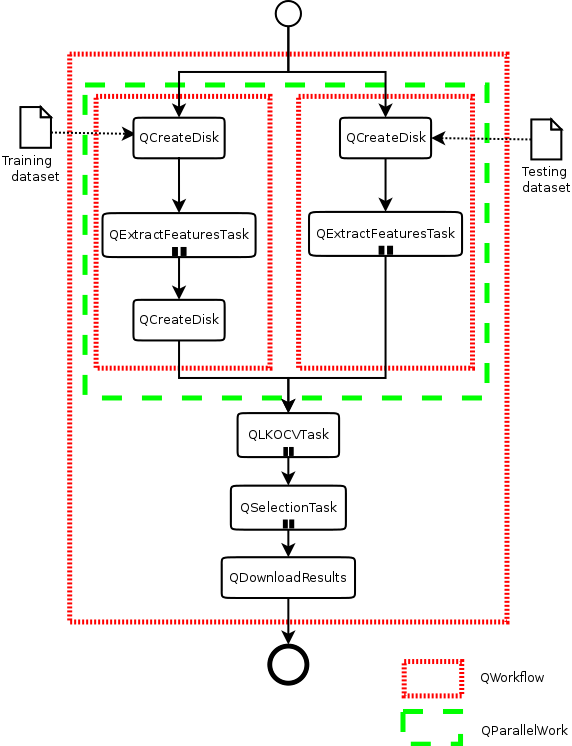
\includegraphics[scale=0.4]{Figures/implementation_vertical.png}
\caption{A possible implementation of the framework using the orchestrator. The green dotted box represents a QParallelWork instance and the red dotted boxes represent QWorkflow instances.}
\label{fig:implementation_diagram}
\end{figure}
\begin{mdframed}[backgroundcolor=LightGray,topline=false, bottomline=false,leftline=false, rightline=false]
\inputminted[baselinestretch=1, fontsize=\scriptsize]{python}{selection.py}
\end{mdframed}
\captionof{figure}{Source code of the proposed implementation.}
\label{fig:implementation_code}
\section{Experimental evaluation} \label{Proof-of-concept}

Show the learning curves.

Show the runtimes.


\section{Conclusion} \label{Conclusion}

[Todo: enrich the monitoring process of the orchestrator]



\bibliographystyle{./IEEEtran}
\bibliography{acoustic}




% that's all folks
\end{document}

